The implementation program main goal is to detect URL category of URL page HTML content. It is made by combining Natural Language Processing(NLP) and Machine Learning(ML) which are described in the Approach sections(links). 

The implementation part consists of these sections:

\begin{enumerate}
    \item {The data set of URLs list}
    \item {Data set creation using NLP techniques}
    \item {Data preprocessing}
    \item {Data training using ML techniques}
    \item {Results and conclusions}
\end{enumerate}


The goal of the project is to solve the URL categorization task using a supervised classification algorithm and using a database with a large number of categorized websites. A supervised classified
should be learned to predict the category a web page belongs to.



\subsection{Data preprocessing}

The one of the most important things solving Machine Learning kind of problems is valid data set source which is required for creating testing and training data sets which are required for training and testing Machine Learning model.

The data set of this problem is available at \href{https://www.figure-eight.com/data-for-everyone/}{Data For Everyone data set lists}. The data set contains 31086 different URLs with 81 attributes. Since the data set has a lot of attributes and few of them will be used in the implementation project, attributes could be represented in this kind of manner:
\begin{itemize}
    \item \textit{unit id}
    \item \textit{golden}
    \item \textit{unit state}
    \item \textit{trusted judgments}
    \item \textit{trusted judgments at}
    \item \textit{main category}
    \item \textit{main category:confidence}
    \item \textit{sub category: Each category}
    \item \textit{sub category: Each category:confidence}
    \item \textit{url}
\end{itemize}

It is an enormous data set and all attributes is barely useful for the implementation problem, the size of data set attribute should be reduced. For the implementation part problem, 3 attributes must be extracted, other attributes should be excluded since they have no impact to the ML model creation. 

List of attributes that are extracted for implementation part:
\begin{enumerate}
    \item \textbf{main\_category} : Attribute describes URL main category.
    \item \textbf{main\_category:confidence} : Attribute describes a probability of accuracy of the URL main category. Since URLs could have a lot of sub-categories it provides information about the most likely main category.
    \item \textbf{url} : Attribute provides URL address of the web page.
\end{enumerate}

\label{sec:categoriesSet}
The data set consist of 25 categories:
\begin{table}[H]
    \begin{tabular}{| l | l | l | l |}
        \hline
         Adult & Finance & News \& Media & Arts \& Entertainment   \\ \hline
         Food \& Drink & People \& Society & Automotive & Gambling   \\ \hline
         Pets \& Animals & Beauty \& Fitness & Games & Reference   \\ \hline
         Books \& Literature & Health & Science & Business \& Industry  \\ \hline
         Home \& Garden & Shopping & Career \& Education & Internet \& Telecom  \\ \hline
         Sports & Computer \& Electronics & Law \& Government & Travel\\ \hline
    \end{tabular}
\captionof{table}{The table of all possible categories} 
\label{table: categories_table}
\end{table}


The primary data is not enough to determine in which category given URL belongs it needs some data preprocessing in order to make a vector and label set for Machine Learning algorithms. 

Data preprocessing consist of 6 major steps:
\begin{enumerate}
    \item Website scraping and text parsing
    \item Text tokenization
    \item Removing stop words and normalizing text
    \item Website language determination
    \item Words frequency
    \item Chunk words
\end{enumerate}

The whole image of the processes could be seen in the figure \ref{fig:dataset_creation}:
\begin{figure}[H]
\centering
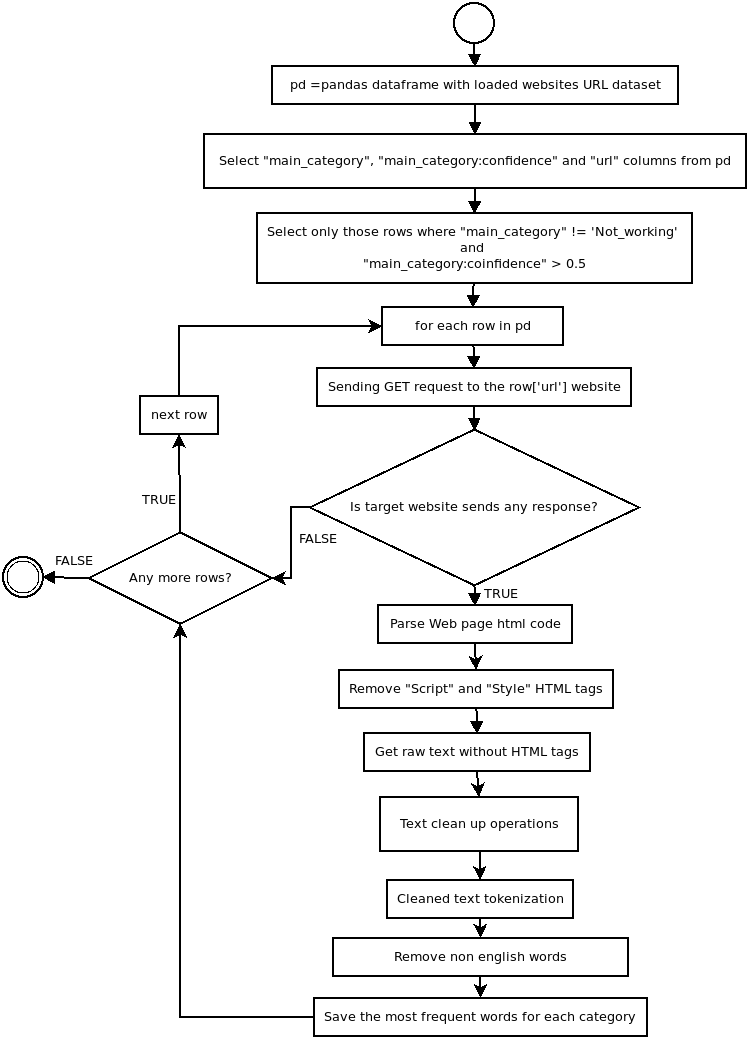
\includegraphics[width=0.8\textwidth]{Pictures/dataset_creation.png}
\caption{\label{fig:dataset_creation}{}Diagram of operations in the data preprocessing}
\end{figure}

Figure \ref{fig:dataset_creation} represents steps that performs data downloading, data filtering and data clean up operations. Since there are a lot of process in this algorithm, in this implementation part each process would be described separately in more depth. 

\subsubsection{Website scraping and text parsing}

The first process is to analyze website and download its content. Every website is build up using HTML language as a core code and the additional design and performance features are added using CSS and JavaScript tools.

The category of the website determines website content. The content is written in the HTML programming language using special tags for displaying information for a user. The main goal of this process is to download the content and parse only necessary text which would be useful for this project. 

This section consist of two parts:
\begin{enumerate}
    \item \textbf{Downloading website content}
    
    Each website content is downloaded by sending GET request using python library \href{https://docs.python.org/3/library/urllib.html}{Urlib}. This library allows to perform GET request to the website and tracks it response.
    
    The expected response from the website is HTML code including Cascading Style Sheets(CSS) and JavaScript(JS) codes. However some websites have security features from scrapping programs, so it is not always possible to get content information from the website. Each website could see the program request header and determine that the request is not performed by the ordinary user and in this case some websites do not respond with the proper information.
    
    Before sending an GET request to the website, the request headers properties are changed to the more likely normal browser properties in order to prevent websites for returning inappropriate response with the HTML content. Also the timeout of the request headers is set to the 15 seconds in order to make some additional time for website response. 
    
    The website is skipped if it is not responding to the GET request
    
    \item \textbf{Website content text parsing}
    
    Website response contains HTML code where the necessary text is stored. There are no need to store text within HTML tags so the other step is to leave only text by excluding HTML tags. This is made by using python library \href{https://pypi.org/project/beautifulsoup4/}{beautifulsoup}. Text parsing consist of these steps:
    \begin{enumerate}
        \item Parse text into beautiful soup object for text filtering and manipulation properties
        \item Filter out CSS and JavaScript content. CSS language is additional tool for improving HTML design which is marked with \textit{<style>} HTML tag and JavaScript is programming language for website behaviour which is marked with \textit{<script>} HTML tag. These elements usually do not contain any useful information so these HTML tags are removed by using beutiful soup function \textit{decompose()}
        \item Text of remain HTML code is extracted by removing HTML tags. HTML tags are removed by using beautiful soup function \textit{get\_text()}
        \item New lines symbols \textit{\n} are removed from the text
        \item The extracted text is stripped in order to remove empty symbols in the text
        \item Every word is joined to the text string by a new line
    \end{enumerate}
\end{enumerate}


\subsubsection{Text tokenization}

The plain text of the website content is not proper format for this project because there is a small probability that the text would be the same among different websites with the same category. However the probability is much bigger that the separated words would more likely to be similar among other website with the same category. This is the reason why the text should be split up to the tokens which would perform plays an important role into project development. 

The parsed text of the website is split up into tokens by using regular expression word tokenizer. Regular expression tokenizer is expressed by this regular expression query: 


\verb/((?<=[^\w\s])\w(?=[^\w\s])|(\W))+$/.

Regular expression symbols explanation:
\begin{description}
    \item \verb/?/ A question mark matches zero or one of the preceding character, class, or sub-pattern. 
    \item \verb/<?=/ Is a positive lookahead, a type of zero-width assertion. What it's saying is that the captured match must be followed by whatever is within the parentheses but that part isn't captured.
    \item \verb/\/ Classes of characters: The square brackets enclose a list or range of characters (or both).
    \item \verb/^/ May appear at the beginning of a pattern to require the match to occur at the very beginning of a line.
    \item \verb/\W/ Matches any single "word" character, namely alphanumeric or underscore.
    \item \verb/\s/ Matches any single white space character, mainly space, tab, and newline (`r and `n). Conversely, capital \S means "any non-white space character". 
    \item + A plus sign matches one or more of the preceding character, class, or sub-pattern.
\end{description}
This regular expression is passed to the \href{https://www.nltk.org/_modules/nltk/tokenize/regexp.html}{nltk python library RegexpTokenizer} function giving an plain text as parameter and it converts plain website text into tokens.

When the text is tokenized, each token word is converted to the lower case. This is made because upper and lower cases have different ASCII codes, so the computer the same words with different ASCII codes treats words as different despite that the words have the same meaning.

\subsubsection{Removing stop words and normalizing text}

\label{sec:stopWords}

Tokens of the website text contains a lot of words, but this does not mean that all the words are proper to use for creating a Machine Learning model. At this point tokens could consist of stop words and random symbols and word could be written in a different grammar forms(singular and plural). These words take a lot of volume in the data, so the volume should be reduced by performing text normalization operations such as \textbf{Removing stop words} and \textbf{Words lemmatization}.


The full image of this process could be seen in a implementation code flowchart figure(\ref{fig:stop_lemma_text}):
\begin{figure}[H]
    \centering
    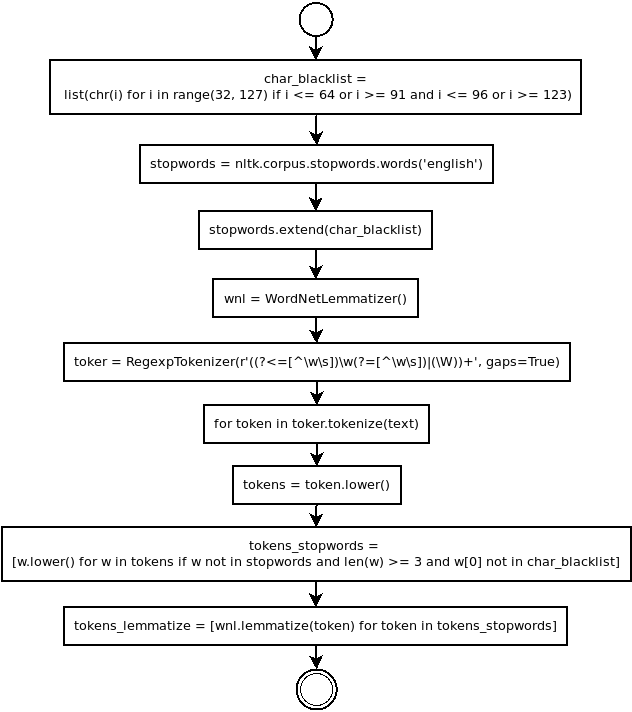
\includegraphics[width=1\textwidth]{Pictures/stop_lemma_text.png}
    \caption{\label{fig:stop_lemma_text}{} An algorithm for processing stop words exclusion and words lemmatization }
\end{figure}

\begin{enumerate}
    \item \textbf{Removing stop words}
    
    Stop words are considered to be common words in a human language which do not provide lots of information by using itself. Tokens contains a list of words that means that they are not connected to the each other and some words by itself do not provides useful information. This is the reason why these words should be removed from the token list because they could confuse the model since most likely every category would contain the same set of words (stop words).
    
    English language is considered of having around 180 stop words. The stop words list database could be found on the internet but for this project \href{https://www.nltk.org/book/ch02.html}{stopwords.words('english')} function which contains 179 commonly used english language stop words. 
    
    
    The main goal of this process is to make sure that the words in the tokens would be meaningful as much as possible, so the additional rules of stop words determination is added. The words with length less than 3 is also considered as as stop words because in english language there are not many words that would contains meaningful information. This is done in order to prevent random symbols that is not determined as words in the english language. The list of these kind of random symbols is made by using \href{http://www.asciitable.com/ASCII} {ASCII(American Standard Code for Information Interchange) table}. The symbols which are in the range of the ASCII table of: [32 : 64], [91 : 96], [123:127] are considered as the stop words. The integer numbers from the range are generated and they are converted to the char symbols that are saved into the list. The list of these symbols are:
    
    ' , !, ", #, \$, \%, \&, \', \(, \), \*, \+, ,, -, ., /, 0, 1, 2, 3, 4, 5, 6, 7, 8, 9, :, ;, <, =, >, ?, @, [, \, ], \^, \_, `, {, |, }, ~'
    
    
    When the stop words list is generated then it is possible to filter out stop words from the tokens. The pseudo algorithm of stop words elimination from the token list:
    \begin{enumerate}
        \item Each word from the token list is iterated
        \item If word is in stop words list then this word is excluded from the token list else the word remains in the token list
    \end{enumerate}
        
    \item \textbf{Words lemmatization}
    
    Words lemmatization  in linguistics is the process of grouping together the inflected forms of a word so they can be analyse as a single item, identified by the word's lemma, or dictionary form. English words grammatically could have 2 forms - singular and plural form. The words core meaning of singular and plural forms remains the same, but the program would treat them as totally different words. The words form is not important for this project problem, so the goal of this process is to have one form for all words that these words would be treated equally according to their core meaning. 
    
    The words lemmatization is done by using english words dictionary of singular and plural forms. The dictionary is build in in the \href{https://www.nltk.org/_modules/nltk/stem/wordnet.html}{nltk python library WordNetLemmatizer} function. The function takes a word as argument and returns a singular form of the word, for example:
    
    
        $children \longrightarrow child$
        
        $word  \longrightarrow words$
    
        $word \longrightarrow word$
        
        
    The examples demonstrates how words forms are converted. The rules of word lemmatization:
    \begin{itemize}
        \item If input word is in a \textbf{singular} form, then output would be an input word in a \textbf{singular} form
        \item If input word is in a \textbf{plural} form, then output would be an input word in \textbf{singular} form
    \end{itemize}
\end{enumerate}

\subsubsection{Website language determination}

There are many human languages with the different words, grammatical features and letters. Each language requires their own approach and analysis, so for this project the one main language is chosen - English language. This language have been chosen, because the majority of websites in the data set contains english language content.

English language considered to be dominant language among websites, because \textbf{10436/19922 (52.38 \%)} are english content websites which are still functioning and the category of these websites is known. 

Language detection could be trivial, because some websites could contain more than one language in their content. For this project the english language was chosen and the language determination was proceed by calculating the ratio of total website words number and website english words number. If the ratio value is more then 50 \%, then the website is considered to be english.


Since some websites could contain more than one language, for this project the english words dictionary is used which is produced by \href{https://www.nltk.org/book/ch01.html}{nltk library english dictionary data set}. The dictionary contains around 171,476 english words which are popular and used every day in colloquial language, 47,156 obsolete english words and 9,500 derivative english words. English words dictionary and website words tokens is enough to calculate ratio of english words and exclude non english words from website tokens list. 
The ratio of english words in the website is not enough, because it could appear websites, where all words are in english, but with small number of instances. These kind of websites are not really useful, because they are lack of words so the websites with less then 10 english words are excluded from the websites list.

Implementation of the language detection could be seen in the code flowchart figure(\ref{fig:detect_lang}):
\begin{figure}[H]
    \centering
    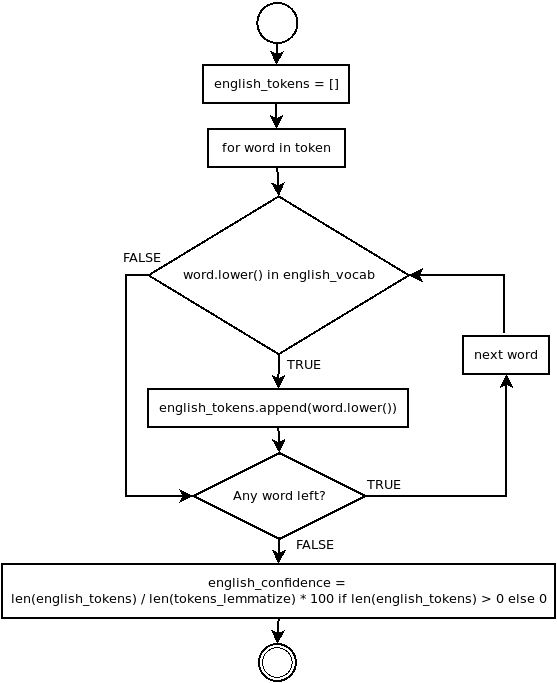
\includegraphics[width=0.65\textwidth]{Pictures/detect_lang.png}
    \caption{\label{fig:detect_lang}{} An algorithm for creating words list }
\end{figure}




Pseudo algorithm for website language determination process:
\begin{enumerate}
    \item A list which would contain all english words is initiated
    \item Each word from website tokens list is iterated
    \item If word appears in the english words dictionary, then word is appended to the english words list(step 1)
    \item Steps 1, 2, 3 are repeated until all words from the token list are iterated
    \item The ratio of english words in the website is calculated by dividing number of english words to total number words in the website token and multiplying by 100 to get percentage representation
    \item If the ratio is less then 50 \% and webpage contains less than 10 english words, then the website considered to be non english content and it would be excluded from the website list
\end{enumerate}
English words which was appended into english words list in step 1 is considered as new words token representation for website since all non english words are excluded.

English websites consist of 101 different top-level domains(TLD). The diversity of the 10 most frequent domains could be seen from the figure(\ref{fig:domain_diversity}) :

\begin{figure}[H]
    \centering
    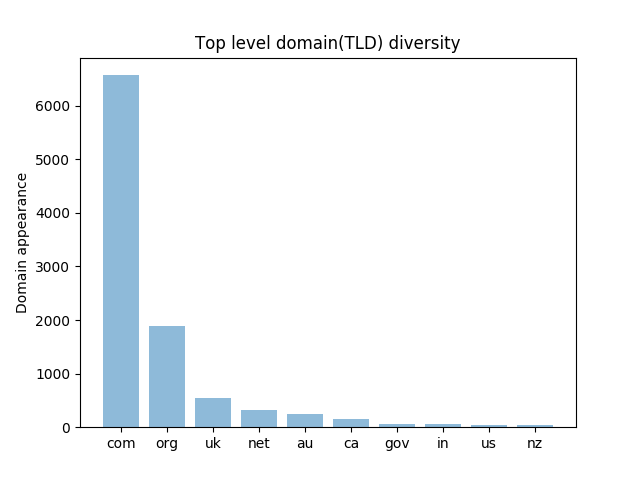
\includegraphics[width=1\textwidth]{Pictures/domain_diversity.png}
    \caption{\label{fig:domain_diversity}{}Top Level Domain(TLD) diversity in the english content websites}
\end{figure}

According to the generated results of TLD diversity in the english content websites (\ref{fig:domain_diversity}) the most frequent domain is \textbf{com} with \textit{6571} instances, the second place took \textbf{org} domain with \textit{1885} instances and the third place took \textbf{uk} domain with \textit{540} instances.

\subsubsection{Words list creation}

In theory every category should contain a different set of words that could represent category itself. At this point a new generated english words token list from the previous subsection contains words for particular website, but not for particular category. One website data is not enough to define the list of the most frequent words in a category, but all websites data are able to create a total word list of all websites for each category where the most frequent words list will be generated after all websites would be analyzed.

The total words list for 24 categories is generated by appending each website words from token list. The dictionary data type is created with shape of \textit{(24, x)} where first dimension represents the name of category and the second dimension represents the set of total words for each category. The value of second dimension is equal x, because each category could contain different number of words. 


Implementation of the total words list creation could be seen in the code flowchart figure(\ref{fig:words_list_creation}):
\begin{figure}[H]
    \centering
    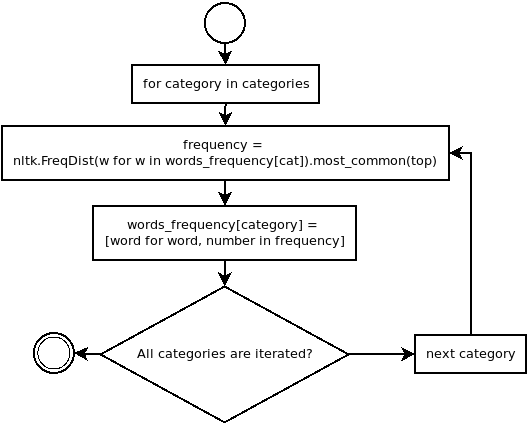
\includegraphics[width=1.05\textwidth]{Pictures/category_words_frequency.png}
    \caption{\label{fig:words_list_creation}{} An algorithm for creating words list }
\end{figure}

Total words list generation pseudo algorithm:
\begin{enumerate}
    \item Each category is iterated from the categories list
    \item If the dictionary do not have key instance of the current category, then dictionary with category key is initialized and it equals for empty list
    \item The dictionary list of category key is extended with a website words token list
    \item Step 1, 2, 3 is repeated until all categories are iterated
\end{enumerate}

Total words list for each category will take a place for creating a list of the most frequent words list for each category.


\subsection{Words frequency model}

This part would cover the most frequent word generation for each category. At this point, the words list should be generated from all websites words tokens including their categories. The words list contains all existing words for each category, so the main part of this section is to determine the most frequent words and sort them ascending mode. This list of the most frequent words would be used for the custom model prediction and also for features generation for Machine learning model.

This section consist of 2 parts:
\begin{enumerate}
    \item \textbf{The most frequently words list for categories} - a list of the most popular words list for each category
    \item \textbf{Chunk words} - methods for detecting chunk words and exclude them from the most frequent words list
\end{enumerate}


\subsubsection{The most frequently words list for categories}


All websites are classified into \hyperref[sec:categoriesSet]{24 categories}. Each category has it is own features which are defined by the words, for example: set of words ['World', 'Business', 'Science', 'Weather', 'Culture', ...] implies that it is probably a set of keywords that may belong to "News & Media" category. Humans could categorize websites content could classify intuitively if website keywords match well known patterns of the category.

The most frequent words list is made from the previously generated word list - all possible words for each category is stored into this list so the main task for this phase is to calculate the frequency of the words and sort them in ascending mode. The vector of the most frequent words list would consist of 2500 words for each category. 

The shape of the most frequent words list: \textit{(24, 2500)} in other words: \textit{categories list, 2500 the most frequent words)}. It is possible to have lower shape of the most frequent words if category all websites contains less then 2500 different words in that case number would be equal a set of words available in a category websites contents.


Implementation of the most frequently words list for categories creation could be seen in the code flowchart figure(\ref{fig:category_words_frequency}):
\begin{figure}[H]
    \centering
    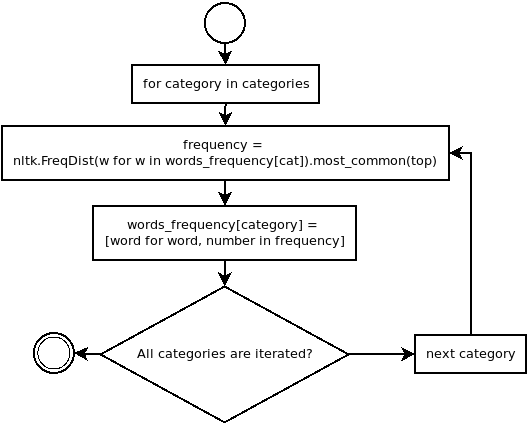
\includegraphics[width=1\textwidth]{Pictures/category_words_frequency.png}
    \caption{\label{fig:category_words_frequency}{} An algorithm for creating the most frequent words list for each category }
\end{figure}

The pseudo algorithm how the most frequent words list is made:
\begin{enumerate}
    \item Each category is iterated from the categories list
    \item Calculating words frequency for each category. The frequency is calculated by using \href{http://www.nltk.org/api/nltk.html?highlight=freqdist}{nltk.FreqDist} function. A function requires a string data type as parameter and it returns the tuple data type of words and their frequency occurrence. The input of the function is words list for each category. Each word from the words list is iterated and passed to the function. In this way the function returns word with it frequency. The words and frequency is sorted in ascending mode. Example of an output of TOP 5 most frequent words in 'Books\_and\_Literature category': $[('book', 5625), ('text', 4094), ('new', 2322), ('novel', 2009)...]$.
    \item Extracting words from the frequent words list. Since the only goal of this process is to generate a list of the most frequent words in the category, the number of words frequency would not be used for the Machine Learning model so only words are extracted and saved in the words frequency list.
\end{enumerate}


\subsubsection{Chunk words}

Generated words frequency list is not perfect because websites could contain a lot of chunk words which are common to all categories. Content of the websites could depend on many factors - current month, political news, casual news or default HTML home page design which includes words like contact or home. Words that are in the TOP 15 the most frequent word list and appears more or equal than 7 categories are called chunk words. 


Implementation of creating and removing chunk words could be seen in the code flowchart figure(\ref{fig:chunk_words}):
\begin{figure}[H]
    \centering
    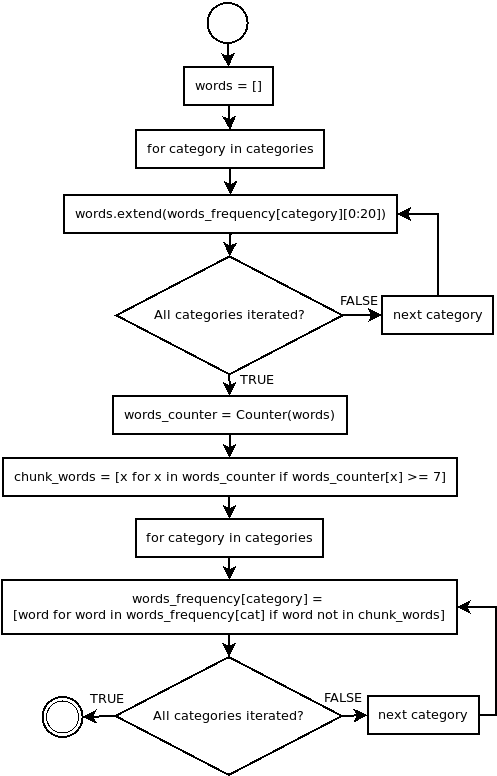
\includegraphics[width=0.65\textwidth]{Pictures/chunk_words.png}
    \caption{\label{fig:chunk_words}{}An algorithm for detecting and removing chunk words }
\end{figure}


The pseudo algorithm for detection of chunk words and chunk words removing process:
\begin{enumerate}
    \item An empty list \textit{words} is created where all top 15 words would be stored
    \item Each category is iterated from the categories list
    \item Top 15 most frequent words in each category is extended to the words list (Step 1)
    \item Steps 2 and 3 are repeated until all categories would be iterated
    \item Words are counted by using \href{https://docs.python.org/2/library/collections.html}{Counter} function
    \item If word appears more or equal than 7 times in different categories, then word is added to the chunk words list
    \item Each category is iterated from the categories list
    \item Words are excluded from the most frequent words list for category by checking if word is in the chunk words list
\end{enumerate}


All chunk words could be seen in the figure(\ref{fig:words_diversity}) :
\begin{figure}[H]
    \centering
    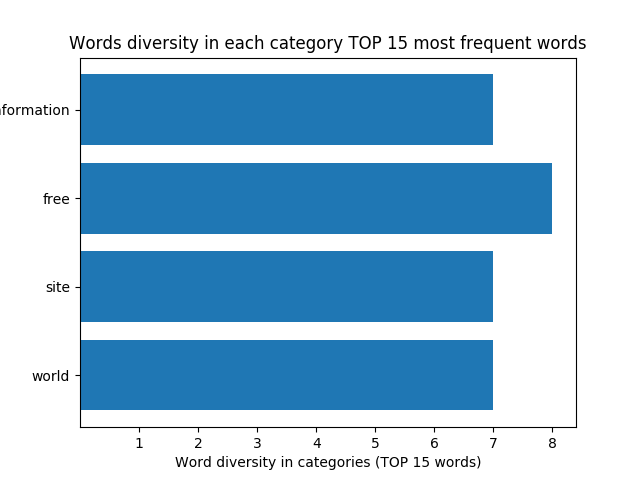
\includegraphics[width=1\textwidth]{Pictures/words_diversity.png}
    \caption{\label{fig:words_diversity}{}An diagram of chunk words diversity in categories }
\end{figure}


According from the most frequent words from each category data generated in December, the bar chart figure(\ref{fig:words_diversity}) shows that there are 4 chunks words: \textit{information, free, site, world}. The word 'free' appeared in a 8 categories while other words appeared in 7 categories. These words are excluded from the most frequent words list.

\subsection{Custom model}

Machine Learning approach is not only way to predict category of the website - other way is to use raw statistics and create a prediction model from already generated words frequency list of each category which was created in the previous section. Since it is known categories most popular words it is possible to find a pattern and predict a category of URL without Machine Learning approach. Custom model creation requires 2 steps:
\begin{enumerate}
    \item Categories features generation
    \item Calculate words weight
\end{enumerate}

This method do not require machine learning approach and it is capable of predicting category of the target website (a website which category will be predicted). Method performance results are much better than usual Machine Learning model. The results and conclusions of custom model are described in the "Results and Conclusion settings" section.

\subsubsection{Categories features generation}

The most frequent words list for categories is used not only for Machine Learning, but also for categories features generation. The method requires a \textit{target website most frequent word list} and \textit{categories most frequent words list} in order to generate the categories features list to determine a target website category. 


The first step of the model creation is gathering the most frequent word list of a target website. The main goal of this process is to create a most frequent words model for each category. Each category would have a list of words that occurred in the target website. At the beginning, each word in the list is equal to the value of 0. By going through each category, if the word occurs in the most frequent words list, then that position the value changes from 0 to 1.

The idea behind this process is to generate vector with the shape: \textbf{(categories number, number of top words in category)}. In implementation part there are  24 different categories and there are tracked top 2500 the most frequent words, so the shape of the list should be: \textbf{(24, 2500)} if there are no chunk words excluded, otherwise it would depend on the particular category most frequent words list length. 

Implementation of this process could be seen in the code flowchart figure(\ref{fig:category_features}):
\begin{figure}[H]
    \centering
    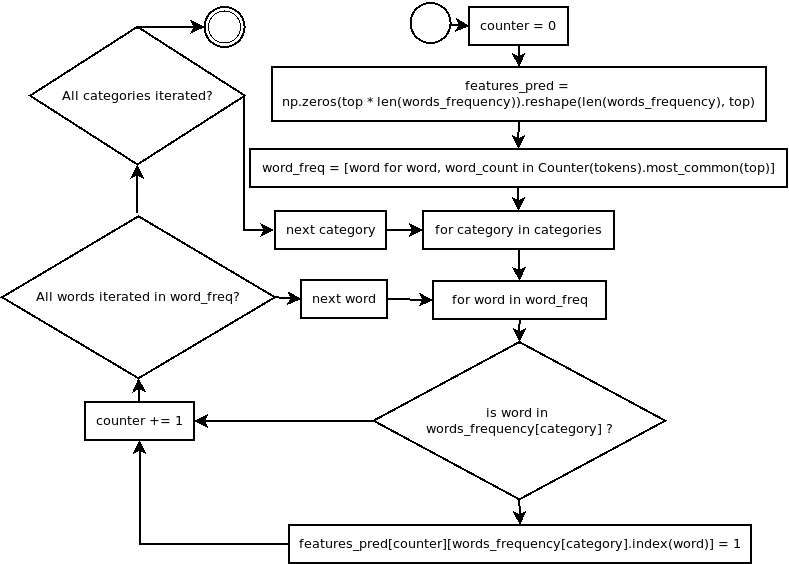
\includegraphics[width=0.9\textwidth]{Pictures/category_features.png}
    \caption{\label{fig:category_features}{}Algorithm of creating the most frequent word vector }
\end{figure}

The Categories features generation for the website pseudo algorithm:
\begin{enumerate}
    \item Creating integer variable "counter" which would track a category index of the list. At the beginning "counter" variable value is equal to 0
    \item Creating a list of the most frequent words: "frequent\_pred". Later on this variable would store of all possible combinations of each category of the most frequent words list.
    
    For each category values of the list are set to 0. 
    
    Variable shape: (25, 2500). First dimension of the list marks category, second dimension of the list marks the top 2500 most frequent words.
    
    \item Storing top 2500 the most frequent words in the "words\_freq" variable. The website all words are counter and sorted in the ascending order from the most frequent word to the least frequent word of top 2500 words. 
    \item Iterating for each category from the categories list
    \item Iterating for each word from the "words\_freq" variable
    \item Checking if the current category most frequent words list contains website current word. If it contains, the index of the word position in the words\_frequency list for current category is saved and used by changing a value of features\_pred[counter][index] from 0 to 1
    \item Step 4 repeats until there no unchecked words left in the word\_freq list
    \item Counter value is auto incremented by 1. This action means that the category is changed to the next one
    \item All steps above are repeated until all categories from the categories list are iterated
\end{enumerate}


In the result of this process the list of the most frequent website words for each category is created. At the beginning the vector is filled with 0 values, but if the word of the website occurs in the category top frequent words list, then the value at the particular position is changed to 1.


In the end of this process, the list of frequent words features is generated for each category. The website words have an impact of a list values. This process generates a list of possible features for each category so the next step is for deciding which feature suits model the best and it is first dimension value would be considered of a target website category.



\subsubsection{Categories weight estimation}


Model feature list which was generated in the previous section should be evaluated in order to extract the category of the target website. The feature estimation is done by processing weight calculation of each category of model feature list and then choosing the max value of the calculated categories which would be considered as category of the target website.


The weight estimation of the model feature list is done by iterating each category list and checking the position whenever values are equal to 1. Every position should have their own weight, because the word frequency list is sorted in ascending mode so words that are close to the list beginning should be more important than those words that are near list end. The main formula of calculating weights of each category is: 
\begin{equation}
    weight\_sum = top - index
\end{equation}
\begin{description}
    \item [weight\_sum] A total sum of all words weights in the category
    \item [top] is a value of how much words are in the most frequent words list which by default value is equal to 2500
    \item [index] An index of where the value of 1 occurred in the category features list
\end{description}


The process of category weight estimation flowchart could be seen in the figure(\ref{fig:category_weight_estimation}):
\begin{figure}[H]
    \centering
    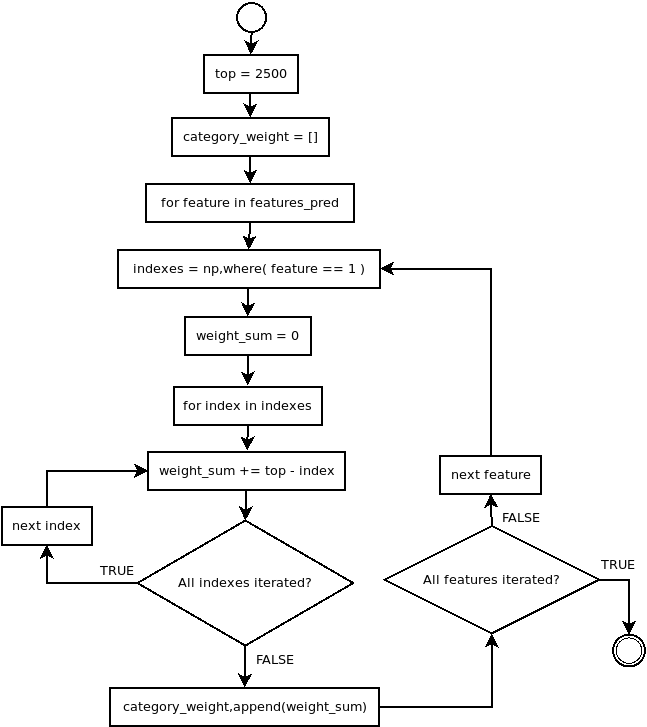
\includegraphics[width=0.85\textwidth]{Pictures/category_weight_estimation.png}
    \caption{\label{fig:category_weight_estimation}{} An algorithm of categories features weight estimation process}
\end{figure}


Category weight estimation pseudo algorithm:


\begin{enumerate}
    \item Creating a list where each category weight sum would be stored. The list is named as \textit{category\_weight}
    \item Iterating for each category features from the categories features list
    \item Getting all positions of the category features list where value is equal to 1. This is done by using \hyperref{https://docs.scipy.org/doc/numpy-1.15.0/reference/generated/numpy.where.html}{np.where()} function. This function requires an input of condition and it generated the position indexes as an output. The condition as an argument to the \hyperref{https://docs.scipy.org/doc/numpy-1.15.0/reference/generated/numpy.where.html}{np.where()} function: $category\_feature == 1$. The function iterates each value of the category features list and if that value is equal to 1, then it stores that value index in the category features list. The output of the function is stored to the \textit{indexes} variable as a numpy data list type.
    \item Creating an integer type variable for storing weight sums for category features list. The variable is named as \textit{weight\_sum}. At the start this variable value is equal to 0
    \item Iterating for each index of \textit{indexes} numpy list
    \item Calculating a weight sum for category features: $weight\_sum += top - index$
    \item Step 6 is repeated until all indexes are iterated
    \item The category features weight is appended into \textit{category\_weigh} list
    \item Steps 2, 3, 4 ,5, 6, 7, 8 are repeated until all categories features are iterated
\end{enumerate}


The main point of this process is to generate a list of all weights for each category features. That list is named as \textit{category\_weight}. At this point the main task is to track the category from the categories features list of the highest weight sum by using \hyperref{https://docs.python.org/3/library/functions.html}{max()} function which returns the highest value in the list. As an input function requires a list and as an output it returns the highest value in the input list. The output value of the highest category features weight sum is indicating website category by using \hyperref{https://docs.python.org/3/library/array.html#array.array.index}{index()} function which returns the index of the input value: $category\_index = category\_weight.index(max(category\_weight))$





\subsection{Machine Learning}


In this section Machine learning algorithms would be trained and tested using by already created the most frequent words list for categories, websites words data and websites categories. The main point of this section is to create a fully working Machine Learning model which would be able to predict a website category without no human interaction for the primary data set.

This is done by processing 4 steps:
\begin{enumerate}
    \item Features and labels creation
    \item Machine Learning models training
    \item Models performance evaluation
\end{enumerate}

\subsubsection{Features and labels creation}

Machine learning algorithms models requires a proper form of data which is the main key of the successful performance of Machine Learning models. At this point the data is almost set up properly - the most frequent words list for categories is created which would help in creating a features and labels for Machine Learning model. Features and labels definitions:
\begin{description}
    \item [Features] are attributes or properties shared by all of the independent units on which analysis or prediction is to be done. 
    
    In this project the features would be considered to be binarized websites most frequent words lists according to the most frequent words list for category list. If a target website most frequent words list values are in the most frequent words list for specific category list, then the value in the most frequent website words list is changed 1 in a position of a word, otherwise value is set to 0.
    
    
    Data set contains the categories of all websites, so in this case it is known which category of the most frequent words list for categories has to be used. 
    \item [Labels] are the final output.
    
    In this project labels are the categories of websites. Since the data set contains all categories of websites so the main task is to track them properly and match them with the features that Machine Learning model would know category of particular website feature set.
\end{description}


The process of features and labels creation for Machine Learning model flowchart could be seen in the figure(\ref{fig:features_labels_creation}):
\begin{figure}[H]
    \centering
    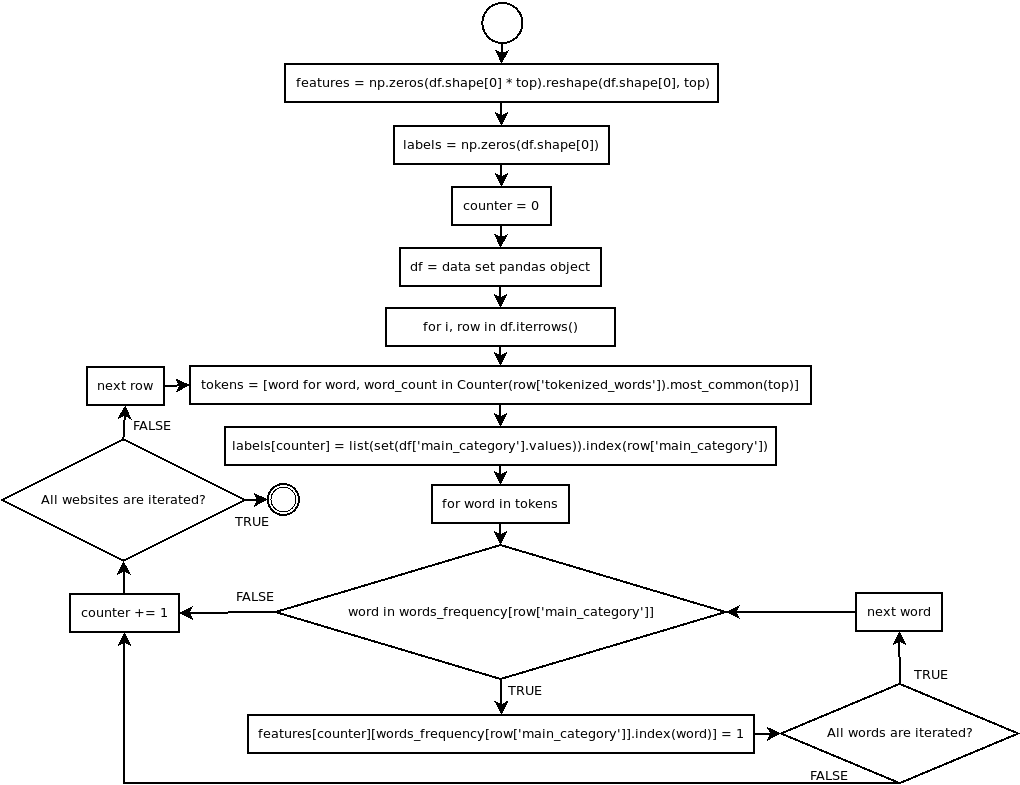
\includegraphics[width=1.085\textwidth]{Pictures/features_labels_creation.png}
    \caption{\label{fig:features_labels_creation}{} An algorithm of features and labels creation}
\end{figure}


Features and labels creation pseudo algorithm:
\begin{enumerate}
    \item List named \textit{features} is created for storing websites features. The features list has a shape of \textbf{(english website length in the data set, top)} which is equals to \textbf{(10436, 2500)} by using december websites data set.
    \item List named \textit{labels} is created for storing websites labels. The labels list has 1-dimensional shape of \textbf{(english website length in the data set)} which is equals to \textbf{(10436)} by using december websites data set.
    \item Integer variable \textit{counter} is created for tracking an index of \textit{labels} list and 1-dimension of \textit{features} list. At the beginning this variable is set to be equal 0
    \item Iterating for each website(\textit{row}) and their position(\textit{i}) in the december websites data set
    \item Defining \textit{labels} list value in the position of \textit{counter}. The category of the website is saved into \textit{labels} list of \textit{counter} position
    \item Iterating for \textit{word} in website token list
    \item Checking if \textit{word} is in the most frequent words list for the current category - if it is true, then \textit{features} list value in 1-dimensional position of \textit{counter} and 2-dimensional position of word in the most frequent words list for current category is set to 1
    \item Steps 7 is repeated until all words are iterated from a website token list
    \item \textit{counter} value is auto incremented by 1
    \item Steps 5, 6, 7, 8, 9 are repeated until all websites are iterated from the december websites data set 
\end{enumerate}


Features and labels are the main data that would be fit to Machine Learning models. However it is a bad practise to use all this data on training machine learning models because of these factors:
\begin{enumerate}
    \item Testing machine learning model. If all data would be used for machine learning model training, then how to be sure how well the model is performing in predicting data set if there are no testing data? Testing data is an indicator of how well machine learning model is performing.
    \item Over fitting problem. Over fit is when your training model is too precise and doesn't generalize on the problem you try to solve. In other words it is too fit for the training, and the training alone, so that it cannot solve/predict a different data set. 
\end{enumerate}

These factors are the reason why features and labels data should be split into \textbf{training} data and \textbf{testing} data. 

At first features and labels data are shuffled by using \href{https://scikit-learn.org/stable/modules/generated/sklearn.utils.shuffle.html}{sklearn.utils.shuffle(*arrays, **options)} function. It shuffles arrays or sparse matrices in a consistent way. Function main argument is features and labels data sets which should be shuffled.


The next step of the shuffled data create training and testing data sets by using \href{https://scikit-learn.org/stable/modules/generated/sklearn.model_selection.train_test_split.html}{sklearn.model_selection.train_test_split(*arrays, **options)} function. This function splits arrays or matrices into random train and test subsets by proportion of 67 \% of total data to training data, and 33 \% of remaining data to the testing data.  


\subsubsection{Machine learning models creation}


Building machine learning models from the scratch requires a lot of time and advanced knowledge about concepts of a particular machine learning model parameters implementations. Machine learning models for implementation part would be created by using Machine learning libraries where a lot of models are already build in. Models are created by using \href{https://scikit-learn.org/stable/}{scikit-learn}  library for python programming language. scikit-learn python library has build in already prepared ready to use machine learning models.


In the implementation part there are created 2 different approach supervised machine learning classifiers types:
\begin{enumerate}
    \item \textbf{Logistic Regression (LR)}
    
    Logistic regression model is created by using \hyperref{https://scikit-learn.org/stable/modules/generated/sklearn.linear_model.LinearRegression.html}{sklearn.linear_model.LinearRegression} library. Fundamentals of the Logistic Regression model are described in the Logistic regression section(\ref{sssec:logistic_regression})
    
    \item \textbf{Linear Support Vector Classification (LSVC)}
    
    Linear Support Vector Classification is one of the branch of Support Vector Machine (SVM) classification model in other words - they are different implementation of the same algorithm. 
    
    The difference between LSVC and SVM: A regular SVM with default values uses a radial basis function as the SVM kernel while LSVC uses a linear kernel for the basis function. That makes LSVC model much less tunable and is basically just a linear interpolation.
    
    Linear Support Vector Classification is created by using \hyperref{https://scikit-learn.org/stable/modules/generated/sklearn.svm.LinearSVC.html}{sklearn.svm.LinearSVC} library with default parameters. LSVC parameters are almost identical as Logistic regression model, except:
\end{enumerate}

Each model has their properties that would have an impact to the model performance. In Logistic Regression and Linear Support Vector Classification shares almost identical parameters. Some of the models parameters description:
\begin{itemize}
    \item \textit{C = 1.0}. C parameter is inverse of regularization strength. Smaller values of C specify stronger regularization. This variable value must be positive. C value is set to 1.0
    \item \textit{class\_weight = None}. Weights associated with classes in the form \{class\_label: weight\}. This value is set up to 'None', because all classes supposed to have at least one weight
    \item \textit{penalty = 'l2'}. Used to specify the norm used in the penalization. L2 penalty indicates that model uses \textit{Ridge Regression} regularization technique.
    \item \textit{dual}. Dual or primal formulation. Dual formulation is only implemented for l2 penalty with liblinear solver. Prefer dual = False when n\_samples > n\_features. In \textbf{Logistic Regression} model dual parameter is set to False, while in \textbf{Linear Support Vector Classification} model dual parameter is set to True.
    \item \itemit{Fit\_intercept = True}. The intercept is the expected mean value of features when all labels are equal to constant value.
    \item \itemit{intercept\_scaling = 1}. Intercept scaling is used to lessen the effect of regularization on synthetic feature weight.
    \item \itemit{max\_iter = 100}. Maximum number of iterations taken for the solvers to converge.
    \item \itemit{random\_state = None}. The seed of the pseudo random number generator to use when shuffling the data
    \item \itemit{tol = 0.0001}. Tolerance for stopping criteria
    \item \itemit{warm\_start = False}. When set to True, reuse the solution of the previous call to fit as initialization, otherwise, just erase the previous solution
\end{itemize}


The last step is to train created Machine Learning models in order to classify websites. This is done by passing generated training features set and training labels set to the \href{https://scikit-learn.org/stable/modules/generated/sklearn.linear_model.LinearRegression.html}{fit method}. Fitting models to the training data is essentially the training part of the modeling process. It finds the coefficients for the equation specified via the algorithm being used. 

Machine learning models after fitting procedure could predict category of the website. The results of prediction may concern of how well data was prepared and also what kind of Machine Learning algorithm was chosen. The prediction is done by using \href{https://scikit-learn.org/stable/tutorial/statistical_inference/supervised_learning.html}{Supervised learning predict function}. This function input is test features set and it returns a labels set of a given features. 

\subsubsection{Models performance evaluation}

Models performance evaluation score is a result of how well models are trained. Evaluation process is performed using 2 different data sets with different websites list. First data set is the original data set from where training/testing features/labels set were created. Second data set is custom made which contains english language websites links with labeled categories.

\begin{enumerate}
    \item \textbf{Models performance evaluation using original data set}.
    
    Primary data set allows evaluate performance for three different parameters: \textif{Precision score, Recall score and F1-score}. Scores evaluations are made for 2 models: Linear Regression model and Linear Support Vector Machine model. 
    
    Since models solves multi-class machine learning approach, because labels consist of 25 different categories, evaluations methods are applied on each category.
    
    \pagebreak
    \textbf{Logistic Regression} model prediction evaluation analysis:

    \begin{table}[H]
        \centering
        \begin{tabular}{l|c|c|c|}
            \hline
            \multicolumn{1}{c}{}  & \multicolumn{3}{|c|}{Logistic Regression}\\\cline{2-4}
            \textbf{Category} & \multicolumn{1}{l|}{\textbf{precision}} & \multicolumn{1}{l|}{\textbf{recall}} & \multicolumn{1}{l|}{\textbf{f1-score}} \\ \hline
            Recreation\_and\_Hobbies & 0.98 & 0.86 & 0.91 \\ \cline{2-4} 
            Food\_and\_Drink & 0.84 & 0.86 & 0.85 \\ \cline{2-4} 
            News\_and\_Media &  0.86 & 0.92 & 0.89  \\ \cline{2-4} 
            Travel & 0.87 & 0.66 & 0.75  \\ \cline{2-4} 
            Career\_and\_Education & 0.93 & 0.80 & 0.86 \\ \cline{2-4} 
            Home\_and\_Garden & 0.88 & 0.86 & 0.87 \\ \cline{2-4} 
            Internet\_and\_Telecom & 0.87 & 0.81 & 0.84 \\ \cline{2-4} 
            Gambling & 0.80 & 0.90 & 0.85 \\ \cline{2-4} 
            Books\_and\_Literature & 0.87 & 0.95 & 0.91 \\ \cline{2-4} 
            Science & 0.95 & 0.88 & 0.91 \\ \cline{2-4} 
            Health & 0.82 & 0.59 & 0.69  \\ \cline{2-4} 
            Autos\_and\_Vehicles & 0.94 & 0.89 & 0.92 \\ \cline{2-4} 
            Finance & 0.80 & 0.86 & 0.83 \\ \cline{2-4} 
            Sports &  0.87 & 0.85 & 0.86 \\ \cline{2-4} 
            Adult & 0.81 & 0.83 & 0.82 \\ \cline{2-4} 
            Pets\_and\_Animals & 0.92 & 0.90 & 0.91 \\ \cline{2-4} 
            Business\_and\_Industry & 0.80 & 0.90 & 0.85 \\ \cline{2-4} 
            People\_and\_Society & 0.83 & 0.26 & 0.40 \\ \cline{2-4} 
            Law\_and\_Government & 0.89 & 0.87 & 0.88 \\ \cline{2-4} 
            Beauty\_and\_Fitness & 0.94 & 0.91 & 0.93 \\ \cline{2-4} 
            Arts\_and\_Entertainment & 0.76 & 0.79 & 0.78 \\ \cline{2-4} 
            Games & 0.88 & 0.81 & 0.84 \\ \cline{2-4} 
            Reference & 0.85 & 0.76 & 0.80 \\ \cline{2-4} 
            Computer\_and\_Electronics & 0.25 & 0.11 & 0.15 \\ \cline{2-4} 
            Shopping &  0.94 & 0.85 & 0.89 \\ \cline{2-4} 
        \end{tabular}
        \caption{Logistic regression model performance evaluation for each category}
        \label{table: lr_table}
    \end{table}
    
    Logistic regression model evaluation scores table (\ref{table: lr_table}) indicates that the most positive predictions (\textit{precision score}) model made on "Recreation\_and\_Hobbies" category with \textbf{0.98 precision score}; category of the highest actual positives identification proportion (\textit{recall score}) is "Books\_and\_Literature" with  \textbf{0.95 recall score}; category of the highest harmonic mean of precision and recall scores is "Beauty\_and\_Fitness" with  \textbf{0.93 f1 score}.
    
    Logistic Regression model overall mean scores for all categories:
    \label{sssec:lr_overall}
    \begin{itemize}
        \item Accuracy score:  0.85
        \item Precision score: 0.85
        \item Recall score: 0.79
        \item F1 score: 0.81
    \end{itemize}
    
    
    Logistic Regression model confusion matrix heat map for each category (\ref{fig:lr_confusion_matrix}):
    \begin{figure}[H]
        \centering
        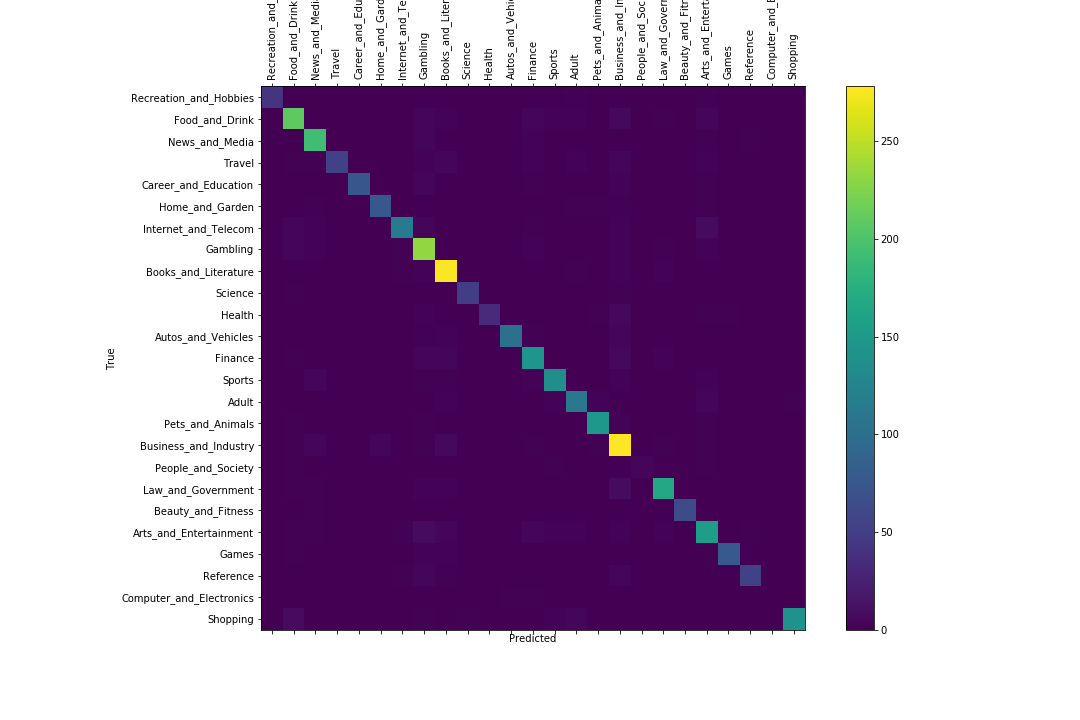
\includegraphics[width=1.2\textwidth]{Pictures/lr_confusion_matrix.png}
        \caption{\label{fig:lr_confusion_matrix}{} Confusion matrix of Logistic Regression model}
    \end{figure}
    
    \pagebreak
    \textbf{Linear Support Vector Machine} model prediction evaluation analysis:
    
    \begin{table}[H]
        \centering
        \begin{tabular}{l|c|c|c|}
            \hline
            \multicolumn{1}{c}{}  & \multicolumn{3}{|c|}{Linear Support Vector Machine}\\\cline{2-4}
            \textbf{Category} & \multicolumn{1}{l|}{\textbf{precision}} & \multicolumn{1}{l|}{\textbf{recall}} & \multicolumn{1}{l|}{\textbf{f1-score}} \\ \hline
            Recreation\_and\_Hobbies & 0.78 & 0.80 & 0.79 \\ \cline{2-4} 
            Food\_and\_Drink &  0.81 & 0.78 & 0.79\\ \cline{2-4} 
            News\_and\_Media &  0.81 & 0.87 & 0.84  \\ \cline{2-4} 
            Travel & 0.79 & 0.54 & 0.64  \\ \cline{2-4} 
            Career\_and\_Education & 0.83 & 0.72 & 0.77 \\ \cline{2-4} 
            Home\_and\_Garden & 0.79 & 0.84 & 0.8 \\ \cline{2-4} 
            Internet\_and\_Telecom & 0.76 & 0.72 & 0.74 \\ \cline{2-4} 
            Gambling & 0.76 & 0.83 & 0.79 \\ \cline{2-4} 
            Books\_and\_Literature & 0.86 & 0.88 & 0.87  \\ \cline{2-4} 
            Science & 0.86 & 0.86 & 0.86 \\ \cline{2-4} 
            Health & 0.62 & 0.52 & 0.56 \\ \cline{2-4} 
            Autos\_and\_Vehicles & 0.86 & 0.84 & 0.85 \\ \cline{2-4} 
            Finance & 0.76 & 0.78 & 0.77 \\ \cline{2-4} 
            Sports &  0.73 & 0.75 & 0.74 \\ \cline{2-4} 
            Adult & 0.77 & 0.75 & 0.76 \\ \cline{2-4} 
            Pets\_and\_Animals & 0.88 & 0.88 & 0.88 \\ \cline{2-4} 
            Business\_and\_Industry & 0.79 & 0.85 & 0.82 \\ \cline{2-4} 
            People\_and\_Society & 0.36 & 0.21 & 0.27 \\ \cline{2-4} 
            Law\_and\_Government & 0.82 & 0.82 & 0.82 \\ \cline{2-4} 
            Beauty\_and\_Fitness & 0.86 & 0.78 & 0.82  \\ \cline{2-4} 
            Arts\_and\_Entertainment & 0.72 & 0.74 & 0.73 \\ \cline{2-4} 
            Games & 0.71 & 0.73 & 0.72  \\ \cline{2-4} 
            Reference &  0.75 & 0.65 & 0.70 \\ \cline{2-4} 
            Computer\_and\_Electronics &  0.08 & 0.11 & 0.09 \\ \cline{2-4} 
            Shopping &   0.81 & 0.77 & 0.79 \\ \cline{2-4} 
        \end{tabular}
        \caption{Linear support vector machine model performance evaluation for each category}
        \label{table: svm_table}
    \end{table}


     Linear support vector machine model evaluation scores table (\ref{table: lr_table}) indicates that the most positive predictions (\textit{precision score}) model made on "Pets\_and\_Animals" category with \textbf{0.88 precision score}; category of the highest actual positives identification proportion (\textit{recall score}) is "Books\_and\_Literature" and "Pets\_and\_Animals" with  \textbf{0.88 recall score}; category of the highest harmonic mean of precision and recall scores is "Pets\_and\_Animals" with  \textbf{0.88 f1 score}.
    
    Linear support vector machine model overall mean scores for all categories:
    \label{sssec:lsvm_overall}
    \begin{itemize}
        \item Accuracy score: 0.79
        \item Precision score: 0.74
        \item Recall score: 0.72
        \item F1 score: 0.73
    \end{itemize}
    
    
    Linear support vector machine model confusion matrix heat map for each category (\ref{fig:lsvm_confusion_matrix}):
    \begin{figure}[H]
        \centering
        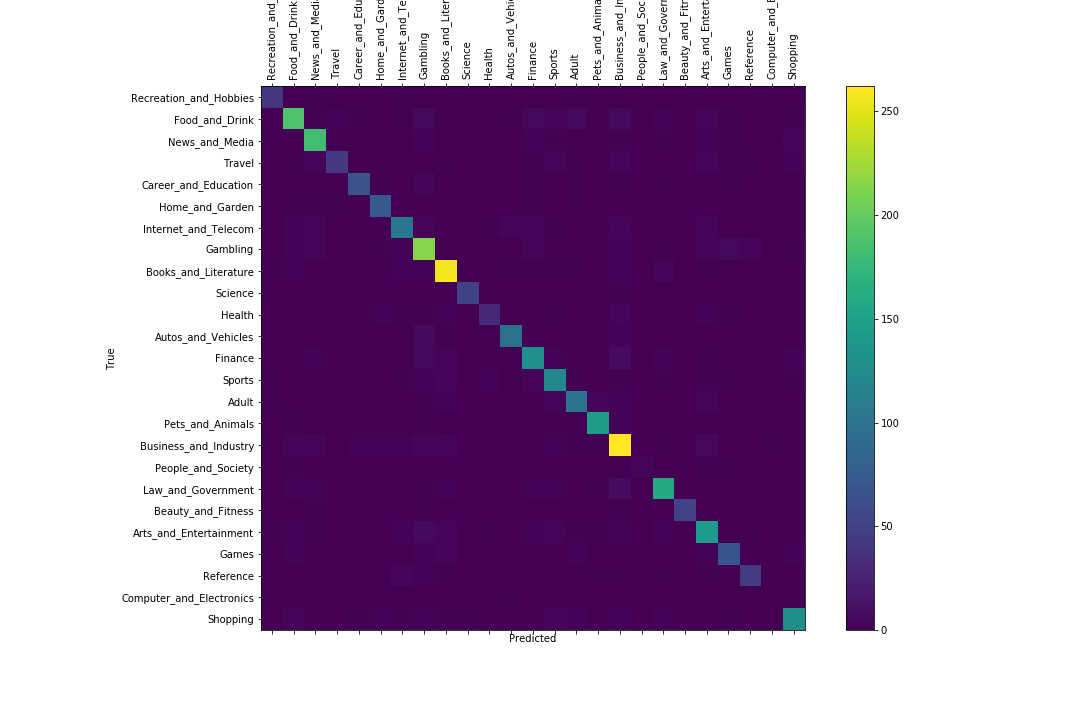
\includegraphics[width=1.2\textwidth]{Pictures/lsvm_confusion_matrix.png}
        \caption{\label{fig:lsvm_confusion_matrix}{} Confusion matrix of Linear Support Vector Machine model}
    \end{figure}
    
    
    Models performance overall evaluation (\ref{sssec:lr_overall}, \ref{sssec:lsvm_overall}) results  implies that model with the best performance for classifying websites categories is \textbf{Linear Regression} model. 
    
\item \textbf{Models performance evaluation using custom made data set}.

Original data set evaluation score is not an final indicator that machine learning models are performing well. The original data set has two serious flaws which could have an impact for final models results. 
\begin{enumerate}
    \item Data set could be outdated. The original data set is created in 2014 year so some of websites content could be changed or not working that leads to another problem that data set classified labels could be changed in the current time.
    \item Classified labels could be wrong. The original data set contains 31086 different websites so to check each website category would consume too much time. Revision of labeled websites would be great to make sure that declared category of particular website is correct
\end{enumerate}

These problems are solved by creating small custom made data set for testing performance on created machine learning models. The custom data set consist of 288 working english websites with human confirmed categories. Each website is iterated and content is download in the same manner of original data set.

On custom model data set is tested my created website categorization model \ref{custom_model} which predicts category of website by creating feature set for each category and calculating weight of the features set. The feature set with the highest weight is considered to be category of the website.

Performance evaluation using custom made data set on my custom model and machine learning models, testing on 286 different websites and there are performance results:

\begin{itemize}
    \item \textbf{Custom model}: 69.5 \% (197 correct predictions of 282)
    \item \textbf{Logistic regression model}: 57.8 \% (163 correct predictions of 282)
    \item \textbf{Linear support vector machine model}: 52.5 \% (148 correct predictions of 282)
\end{itemize}
From given results custom model performance is the best for predicting up to date websites categories. Machine learning models performance is similar - logistic regression manage correctly predict 163 websites categories while linear support vector machine 148 websites categories. According to original data set machine learning models results - linear regression model should perform better than linear support vector machine and that confirms performance results on the custom data set.

\pagebreak
Models performance on predicting each category:

 \begin{table}[H]
        \centering
        \begin{tabular}{l|c|c|c|}
            \hline
            \multicolumn{1}{c}{}  & \multicolumn{3}{|c|}{Custom data set performance evaluation}\\\cline{2-4}
            \textbf{Category} & \multicolumn{1}{l|}{\textbf{Custom model}} & \multicolumn{1}{l|}{\textbf{LR model}} & \multicolumn{1}{l|}{\textbf{LSVM model}} \\ \hline
            Food\_and\_Drink & 6 / 7 : 85.71 \% & 6 / 7 : 85.71 \% & 6 / 7 : 85.71 \% \\ \cline{2-4} 
            News\_and\_Media &  12 / 14 : 85.71 \% & 11 / 14 : 78.57 \% & 11 / 14 : 78.57 \%  \\ \cline{2-4} 
            Travel & 13 / 15 : 86.67 \% & 8 / 15 : 53.33 \% & 7 / 15 : 46.67 \%  \\ \cline{2-4} 
            Career\_and\_Education & 14 / 14 : 100.00 \% & 11 / 14 : 78.57 \% & 9 / 14 : 64.29 \% \\ \cline{2-4} 
            Home\_and\_Garden & 3 / 16 : 18.75 \% & 2 / 16 : 12.50 \% & 2 / 16 : 12.50 \% \\ \cline{2-4} 
            Internet\_and\_Telecom & 3 / 16 : 18.75 \% & 3 / 16 : 18.75 \% & 2 / 16 : 12.50 \% \\ \cline{2-4} 
            Gambling & 9 / 9 : 100.00 \% &  6 / 9 : 66.67 \% & 5 / 9 : 55.56 \% \\ \cline{2-4} 
            Books\_and\_Literature & 7 / 10 : 70.00 \% & 7 / 10 : 70.00 \% & 7 / 10 : 70.00 \% \\ \cline{2-4} 
            Science & 16 / 20 : 80.00 \% & 13 / 20 : 65.00 \% & 11 / 20 : 55.00 \% \\ \cline{2-4} 
            Health & 9 / 11 : 81.82 \% & 6 / 11 : 54.55 \% & 6 / 11 : 54.55 \%  \\ \cline{2-4} 
            Autos\_and\_Vehicles & 13 / 16 : 81.25 \% & 13 / 16 : 81.25 \% & 12 / 16 : 75.00 \% \\ \cline{2-4} 
            Finance & 13 / 19 : 68.42 \% & 12 / 19 : 63.16 \% & 12 / 19 : 63.16 \% \\ \cline{2-4} 
            Sports & 8 / 9 : 88.89 \% & 7 / 9 : 77.78 \% & 5 / 9 : 55.56 \% \\ \cline{2-4} 
            Adult & 8 / 8 : 100.00 \% & 7 / 8 : 87.50 \% & 5 / 8 : 62.50 \% \\ \cline{2-4} 
            Pets\_and\_Animals & 9 / 12 : 75.00 \% & 5 / 12 : 41.67 \% & 5 / 12 : 41.67 \% \\ \cline{2-4} 
            Business\_and\_Industry & 4 / 8 : 50.00 \% & 3 / 8 : 37.50 \% & 3 / 8 : 37.50 \% \\ \cline{2-4} 
            People\_and\_Society & 1 / 1 : 100.00 \% & 1 / 1 : 100.00 \% & 1 / 1 : 100.00 \% \\ \cline{2-4} 
            Law\_and\_Government & 6 / 8 : 75.00 \% & 4 / 8 : 50.00 \% & 4 / 8 : 50.00 \% \\ \cline{2-4} 
            Beauty\_and\_Fitness & 19 / 23 : 82.61 \% & 16 / 23 : 69.57 \% & 14 / 23 : 60.87 \% \\ \cline{2-4} 
            Arts\_and\_Entertainment & 2 / 10 : 20.00 \% & 2 / 10 : 20.00 \% & 2 / 10 : 20.00 \% \\ \cline{2-4} 
            Games & 3 / 6 : 50.00 \% & 2 / 6 : 33.33 \% & 2 / 6 : 33.33 \% \\ \cline{2-4} 
            Reference & 1 / 10 : 10.00 \% & 1 / 10 : 10.00 \% & 1 / 10 : 10.00 \% \\ \cline{2-4} 
            Computer\_and\_Electronics & 12 / 13 : 92.31 \% & 12 / 13 : 92.31 \% & 12 / 13 : 92.31 \% \\ \cline{2-4} 
            Shopping &  6 / 7 : 85.71 \% & 5 / 7 : 71.43 \% & 4 / 7 : 57.14 \% \\ \cline{2-4} 
        \end{tabular}
        \caption{Models performance on predicting each category}
        \label{table: custom_table}
    \end{table}
\end{enumerate}

According to the custom data set performance results(\ref{table: custom_table}) models performance on predicting category the best results are performed on category "Career\_and\_Education" where custom model predicts of 100 \% accuracy; logistic regression model and linear support vector machine model predict on 78.57 \% accuracy. Not all predictions on categories are equal, because there are different websites instances of categories. For example: category "People\_and\_Society" all models predicted at 100 \% accuracy, but this is not quite accurate since there is only 1 website with in the custom data set with that category. To make this evaluation more accurate, the custom data set should be expanded with more websites instances and websites instances on categories number should be equal for all categories.  

